%------------------------------------------------------------------------------
% Beginning of journal.tex
%------------------------------------------------------------------------------
%
% AMS-LaTeX version 2 sample file for journals, based on amsart.cls.
%
%        ***     DO NOT USE THIS FILE AS A STARTER.      ***
%        ***  USE THE JOURNAL-SPECIFIC *.TEMPLATE FILE.  ***
%
% Replace amsart by the documentclass for the target journal, e.g., tran-l.
%
\documentclass{amsart}

%     If your article includes graphics, uncomment this command.
\usepackage{graphicx}

\newtheorem{theorem}{Theorem}[section]
\newtheorem{lemma}[theorem]{Lemma}

\theoremstyle{definition}
\newtheorem{definition}[theorem]{Definition}
\newtheorem{example}[theorem]{Example}
\newtheorem{xca}[theorem]{Exercise}

\theoremstyle{remark}
\newtheorem{remark}[theorem]{Remark}

\numberwithin{equation}{section}

%    Absolute value notation
\newcommand{\abs}[1]{\lvert#1\rvert}

%    Blank box placeholder for figures (to avoid requiring any
%    particular graphics capabilities for printing this document).
\newcommand{\blankbox}[2]{%
  \parbox{\columnwidth}{\centering
%    Set fboxsep to 0 so that the actual size of the box will match the
%    given measurements more closely.
    \setlength{\fboxsep}{0pt}%
    \fbox{\raisebox{0pt}[#2]{\hspace{#1}}}%
  }%
}

\begin{document}

\title{Structural Stability of Random Dynamical Systems}

%    Information for first author
\author{Aviv Bergman}
%    Address of record for the research reported here
\address{Department of Systems and Computational Biology, Albert Einstein College of Medicine, Bronx, New York 10461}
%    Current address
\curraddr{}
\email{aviv@einstein.yu.edu}
%    \thanks will become a 1st page footnote.
\thanks{The first author was supported in part by NSF Grant \#000000.}

%    Information for second author
\author{Raymond S. Puzio}
\address{Department of Systems and Computational Biology, Albert Einstein College of Medicine, Bronx, New York 10461}
%    Current address
\curraddr{}
\email{rsp@novres.org}
\thanks{Support information for the second author.}

%    Information for third author
\author{Cameron Smith}
\address{Department of Systems and Computational Biology, Albert Einstein College of Medicine, Bronx, New York 10461}
%    Current address
\curraddr{}
\email{cameron.smith@med.einstein.yu.edu}
\thanks{Support information for the second author.}

%    General info
\subjclass[2000]{Primary 54C40, 14E20; Secondary 46E25, 20C20}

\date{January 1, 2001 and, in revised form, June 22, 2001.}

\dedicatory{This paper is dedicated to our advisors.}

\keywords{Differential geometry, algebraic geometry}

\begin{abstract}
This paper is a sample prepared to illustrate the use of the American
Mathematical Society's \LaTeX{} document class \texttt{amsart} and
publication-specific variants of that class for AMS-\LaTeX{} version 2.
\end{abstract}

\maketitle

\section{$2 \times 2$ systems}
We call a matrix stable when all its eigenvalues are negative.  For a
$2 \times 2$ matrix, this amounts to the conditions $T < 0$ and $D >
0$ where $T$ and $D$ denote the trace and the determinant.

Suppose we have a stable matrix
$$
\begin{pmatrix}
a & b \\
d & c
\end{pmatrix}
$$
where $a + c < 0$ and $ac > bd$.  We want to know the probability
that, if we resample an element of this matrix, the result will be
stable.  By symmetry, there are two cases to consider; resampling
$a$ is equivalent to resampling $d$ and resampling $b$ is equivalent
to resampling $c$.

Suppose that we resample $b$.  Since the trace does not involve $b$,
that condition will be satisfied automatically and we only need to
examine the determinant.  Thus, we have the inequalities $ac > bd$ and $-1 < b < 1$.  We will consider seperately the cases of $d
< 0$ and $d > 0$.  When $d > 0$, the first condition becomes $ac/d > b$.
Since $b > -1$, this can only be satisfied when $ac/d > -1$, i.e. when $ac > -d$.  In the subcase that $ac < d$, we then have the limits $-1 < b < ac/d$ and in the subcase $ac < d$, we have the limits $-1 < b < 1$.  When $d < 0$, the condition becomes
$ac/d < b$, which is satisfiable when $ac > d$.  In the subcase where $ac > -d$, we have $ac/d < b < 1$ and, in the subcase where $ac < -d$, we have $-1 < b <
1$.

Thus, the probability that a random stable matrix will remain stable
upon resampling $b$ is given as follows:
% \begin{strip}
\begin{align*}
&{\int_{ac>bd \atop a+c<0} da\,db\,dc\,dd\,
  P(ac>b'd, a+c < 0) \over
\int_{ac>bd \atop a+c<0} da\,db\,dc\,dd\,1} = \cr
&{{{1 \over 32} \int_0^1 dd \int_{d > ac > -d} da\,dc \int_{-1}^{ac/d} db \,
({ac \over d} + 1) + {1 \over 32} \int_{0}^{1} dd \int_{ac>d} da\,dc \int_{-1}^{1} db 2 \atop +
{1 \over 32} \int_{-1}^0 dd \int_{-d > ac > d} da\,dc \int_{ac/d}^1 db\, (1
- {ac \over d}) + {1 \over 32} \int_{-1}^{0} dd \int_{ac>-d} da\,dc \int_{-1}^{1} db 2}
\over
{{{1 \over 16} \int_0^1 dd \int_{d > ac > -d} da\,dc \int_{-1}^{ac/d} db\,1
+ {1 \over 16} \int_{0}^{1} dd \int_{ac>d} da\,dc \int_{-1}^{1} db 1} \atop
{+ {1 \over 16} \int_{-1}^0 dd \int_{-d > ac > d} da\,dc \int_{ac/d}^1 db\,1} + {1 \over 16} \int_{-1}^{0} dd \int_{ac>-d} da\,dc \int_{-1}^{1} db 1}}
\end{align*}
% \end{strip}

In order to evaluate the integrals, we begin with the
integrals over $b$, which are particularly easy because none of the
integrands depends upon $b$.  Once we do that and make the change of
variables $d \mapsto -d$ in the second integrals in the numerator and
denominator, we can combine terms and simplify the expression to the
following:
$$
\frac{\int_0^1 dd \int_{ac > d} da\,dc\, 4 + \int_0^1 dd \int_{d > ac > -d} da\,dc ({ac \over d} + 1)^2}{2 \int_0^1 dd \int_{ac > d} da\,dc\, 2 + 2 \int_0^1 dd \int_{d > ac > -d} da\,dc ({ac \over d} + 1)}
$$

\begin{figure}[!ht]
\centering
\noindent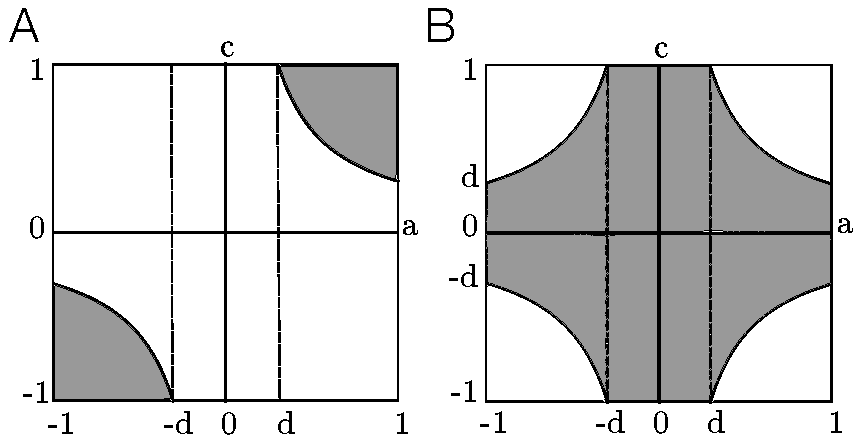
\includegraphics[width=0.5\columnwidth]{fig/2x2-resample-b.pdf}
\caption{{\bf Resampling b.} (A) The region defined by $ac > d$ (B) The region defined by $d > ac > -d$}
\label{fig:2x2-resample-b}
\end{figure}

For $ac > d$ we divide the $a$-axis into two parts indicated in Fig. \ref{fig:2x2-resample-b}A
$$
\int_{ac>d} da\,dc \, f(a,c) = \int_{-1}^{-d} da \int_{-1}^{d \over a} dc \, f(a,c) + \int_{d}^{1} da \int_{d \over a}^1 dc \, f(a,c)$$
for the numerator $f(a,c) = 4$ and the integral is equal to 2. For $d > ac > -d$ we divide the $a$-axis into three parts indicated in Fig. \ref{fig:2x2-resample-b}B
$$
\int_{d > ac > -d} da\,dc \, f(a,c) = \int_{-1}^{-d} da \int_{d \over a}^{- d \over a} dc \, f(a,c) + \int_{-d}^{d} da \int_{-1}^{1} dc \, f(a,c) + \int_{d}^{1} da \int_{-d \over a}^{d \over a} dc \, f(a,c)
% \over {\int_{-1}^{-d} da \int_{d \over a}^{- d \over a} dc + \int {-d}^{d} da \int_{-1}^{1} dc + \int_{d}^{1} da \int_{-d \over a}^{d \over a} dc}
$$
for the numerator $f(a,c) = (\frac{ac}{d} + 1)^2$ and the integral is equal to $\frac{32}{9}$ and for the denominator $f(a,c) = \frac{ac}{d} + 1$ and the integral is equal to $3$. Therefore
$$P\left(\begin{pmatrix}
a & b' \\
d & c
\end{pmatrix} \textrm{stable } \bigg| \begin{pmatrix}
a & b \\
d & c
\end{pmatrix} \textrm{stable } \right) = \frac{25}{36} \approx 0.69.$$

% Thus, our expression becomes
% $$
% {\int_0^1 dd \int_{-1}^{-d} da \int_{-1}^{-d/a} dc\, ({ac \over d} + 1)^2 +
% \int_0^1 dd \int_{-d}^{d} da \int_{-1}^{1} dc\, ({ac \over d} + 1)^2 +
% \int_0^1 dd \int_d^1 da \int_{-d/a}^{1} dc\, ({ac \over d} + 1)^2
% \over
% 2\int_0^1 dd \int_{-1}^{-d} da \int_{-1}^{-d/a} dc\, ({ac \over d} + 1) +
% 2 \int_0^1 dd \int_{-d}^{d} da \int_{-1}^{1} dc\, ({ac \over d} + 1) +
% 2 \int_0^1 dd \int_d^1 da \int_{-d/a}^{1} dc\, ({ac \over d} + 1) }
% $$

Now suppose we resample $a$.  Then we have to satisfy the conditions
$a + c < 0$, $ac > bd$, and $-1 < a < 1$ for fixed values of $b,c,d$.  We will
consider seperately the cases $c > 0$ and $c < 0$.  When $c > 0$, our
inequalities become $a < -c$ and $a > bd/c$.  For these to be
consistent, we must have $-c > bd/c$, or $bd < -c^2$.  In the subcase where $bd < -c$, we have $-1 < a < -c$ and, in the subcase where $-c < bd < -c^2$, we have $bd/c < a < -c$. When $c < 0$, the conditions become $a < -c$ and
$a < bd/c$, which will have a solution as long as $bd/c > -1$, or $bd
< -c$.  In the subcase where $bd < -c^2$, we have $-1 < a < bd/c$ and, in the subcase where $bd > -c^2$, we have $-1 < a < -c$.

Thus, the probability that a random stable matrix will remain stable upon resampling $a$ is given as follows:
\begin{align*}
&\frac{\int_{ac>bd \atop a+c<0} da\,db\,dc\,dd\,
  P(a'c>bd, a'+c < 0)}{\int_{ac>bd \atop a+c<0} da\,db\,dc\,dd\,1} = \\
&\frac{\genfrac{}{}{0pt}{}{{1 \over 32} \int_0^1 dc \int_{bd < -c^2} db\,dd \int_{\max(bd/c,-1)}^{-c} da \,
(-c - \max({bd \over c},-1)}{+
{1 \over 32} \int_{-1}^0 dc \int_{bd < -c} db\,dd \int_{-1}^{\min(-c,
bd/c)} da\, (\min(-c, bd/c) + 1)}}{{1 \over 16} \int_0^1 dc \int_{bd < -c^2} db\,dd \int_{bd/c}^{-c} da\,1
+
{1 \over 16} \int_{-1}^0 dc \int_{bd < -c} db\,dd \int_{-1}^{\min(-c, bd/c)} da\,1}
\end{align*}

\begin{figure}[!ht]
\centering
\noindent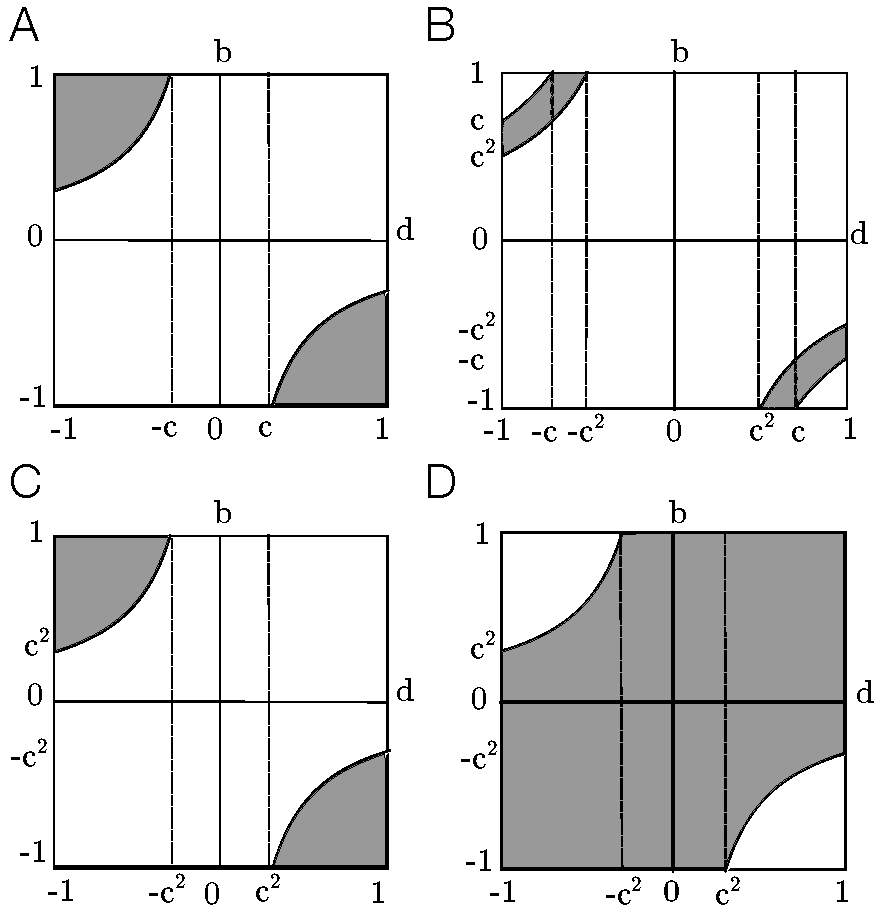
\includegraphics[width=0.5\columnwidth]{fig/2x2-resample-a.pdf}
\caption{{\bf Resampling a.} (A) The region defined by $bd < -c$ (B) The region defined by $-c < bd < -c^2$ (C) The region defined by $bd < -c^2$ (D) The region defined by $bd > -c^2$}
\label{fig:2x2-resample-a}
\end{figure}

For the case $c>0, {bd \over c} < a < -c, bd < -c^2$ we have two possibilities. For $bd < -c$ we have
$$
\int_{-1}^{-c} dd\, \int_{c/d}^1 db\, + \int_c^1 dd\, \int_{-1}^{-c/d} db,
$$
and for $bd > c$
$$
\int_{-1}^{-c} dd\, \int_{-c^2/d}^{-c/d} db\, + \int_{-c}^{-c^2} dd\, \int_{-c^2/d}^{1} db +
\int_{c^2}^{c} dd \int_{-1}^{-c^2/d} db +
\int_{c}^{1}dd\,\int_{-c/d}^{-c^2/d}db.
$$
For the case $c < 0, a < -c, a < bd/c$ we also have two possibilities. For $bd < -c^2$ we have
$$
\int_{-1}^{-c^2} dd\, \int_{-c^2/d}^1 db\, + \int_{c^2}^1 dd\, \int_{-1}^{-c^2/d} db,
$$
and for $bd > -c^2$
$$
\int_{-1}^{-c^2} dd\, \int_{-1}^{-c^2/d} db\, + \int_{-c^2}^{c^2} dd\, \int_{-1}^{1} db +
\int_{c^2}^{1} dd \int_{-c^2/d}^{1} db.
$$

\section{Arbitrary system size}
We call a matrix $M$ stable if all its eigenvalues have negative real
part.  Define the polynomial $p(x) = \det(xI + M)$.  Then, since the
roots of $p$ are minus the eigenvalues of $M$, asking that $M$ be
stable is equivalent to asking that the roots of $p$ all have real
part.  Using some good old fashioned invariant theory, we will
formulate conditions for this to happen in terms of the coefficients of
$p$.

Let us start by fixing some notation.  Suppose that $M$ is of size $n
\times n$.  Denote the coefficients of $p$ as $s_j$ and its roots as
$r_j$, writing $p(x) = x^n + \sum_{k=1}^n s_k x^{n-k} = \prod_{k=1}^n
(x-r_k)$.

Introduce $V$ as the parameter space of all polynomials or degree $n$
with real coefficients.  In other words, $V$ is a real vector space of
dimension $n$ whose coordinates we will identify with the coefficients
$s_k$ of our polynomial.  We now partition this space into regions
corresponding to specific types of polynomials.  Let $R_{abcd}$ be the
subset of $V$ such that $x \in R_{abcd}$ iff the polynomial
corresponding to $x$ has $a$ positive real roots, $b$ negative real
roots, $c$ complex roots with positive real part and $d$ complex roots
with negative real part.  Once we characterize these regions using
invariants, we will have solved the original problem because a matrix
is stable if the point of $V$ corresponding to it lies in a region of
the form $R_{a0c0}$.

Next, we introduce some products:
\begin{align}
D &= \prod_{k=1}^n r_n \cr
\delta &= \prod_{j=1}^{n-1} \prod_{k=j+1}^n (r_1 - r_j)^2 \cr
\Delta &= \prod_{j=1}^{n-1} \prod_{k=j+1}^n (r_1 + r_j) \cr
\end{align}

Since these quantities are invariant under permutation of the roots
$r_j$, they may be expressed as functions of the coefficients $s_j$.
The explicit expressions may be obtained by such techniques as long
division and determinants.

These quantities are of interest because they describe the boundaries
between the regions introduced above.  Suppose that we have a family
of polynomials whose roots are of one type but turn into another type.
There are three ways this could happen:
\begin{itemize}
\item{1.} A real root could go from being positive to being negative
  or vice versa.  For this to happen, we must pass through an
  intermediate value with a zero root.  For that intermediate value,
  we have $D = 0$.
\item{2.} A pair of real roots could turn into a pair of complex roots
  or vice versa.  For this to happen, we must pass through an
  intermediate value with a repeated root.  For that intermediate
  value, we have $\delta = 0$.
\item{3.} A conjugate pair of complex roots could go from having
  positive real part to having negative real part or vice versa.  For
  this to happen, we must pass through an intermediate value in which
  the real part is zero.  For that intermediate value, the two roots
  are imaginary so, bing conjugates, they sum to zero, hence we have
  $\Delta = 0$.
\end{itemize}
\noindent  Thus, we conclude that the boundaries of our regions
$R_{abcd}$ consist of portions of the surfaces $D=0, \delta=0,
\Delta=0$ and we will characterize them by studying these surfaces.

The simplest case is $n=2$.  There we have the regions $R_{2000},
R_{1100}, R_{0200}, R_{0020}, R_{0002}$ and our invariants are $D =
s_2, \delta = s_1^2 - 4s_2, \Delta = s_1$.  The relation between these
is summarized in the following table:
\begin{align}
R_{2000} \qquad &D > 0, \delta > 0, \Delta > 0 \cr
R_{1100} \qquad &D < 0, \delta > 0 \cr
R_{0200} \qquad &D > 0, \delta > 0, \Delta < 0 \cr
R_{0020} \qquad &\delta < 0, \Delta > 0 \cr
R_{0002} \qquad &\delta < 0, \Delta < 0 \cr
\end{align}

Moving to $n=3$, our invariants now look as follows: $D = s_3, \delta
= 18 s_1 s_2 s_2 + s_1^2 s_2^2 - 4 s_2^3 - 4 s_1^3 s_3 - 27 s_3,
\Delta = s_1 s_2 - s_3$.  However, now we can no longer simply use their
signs to distinguish regions.  For instance, consider the regions
$R_{3000}$ and $R_{1200}$.  These both have $D > 0$ and $\delta > 0$
but to tell them apart, we need to note that the region $\delta > 0$
has two connected components and use some auxiliary equalities to
specify which of the components contains our region.  (Looking at the
sign of $\Delta$ will not help here because, while $\Delta > 0$ in the
region $R_{3000}$, it is also positive for some elements of $R_{1200}$
as well.)

% \bibliographystyle{amsplain}
% \begin{thebibliography}{10}

% \bibitem {A} T. Aoki, \textit{Calcul exponentiel des op\'erateurs
% microdifferentiels d'ordre infini.} I, Ann. Inst. Fourier (Grenoble)
% \textbf{33} (1983), 227--250.

% \bibitem {B} R. Brown, \textit{On a conjecture of Dirichlet},
% Amer. Math. Soc., Providence, RI, 1993.

% \bibitem {D} R. A. DeVore, \textit{Approximation of functions},
% Proc. Sympos. Appl. Math., vol. 36,
% Amer. Math. Soc., Providence, RI, 1986, pp. 34--56.

% \end{thebibliography}

\end{document}

%------------------------------------------------------------------------------
% End of journal.tex
%------------------------------------------------------------------------------
